\documentclass{article}
\usepackage{graphicx}
\usepackage{datetime}
\usepackage{geometry}
\usepackage{placeins}
\usepackage{minted}
\usepackage{xcolor}
\usepackage{caption}
\usepackage{lmodern} 
\usepackage[document]{ragged2e}
\usepackage[hidelinks]{hyperref}
\usepackage{enumitem}
\geometry{
 a4paper,
 left=25mm,
 top=25mm,
 }
\captionsetup{hypcap=false} 
\newdateformat{daymonthyear}{\THEDAY .\THEMONTH .\THEYEAR}
\title{
  \centering
  
\includegraphics[width=\textwidth]{images/logo_PWr_kolor_poziom.png}\\
  \fontsize{28pt}{30pt}\selectfont Sprawozdanie 5\\
  \fontsize{14pt}{30pt}\selectfont Ćwiczenie 5.Transmisja WiFi}
\author{Krzysztof Zalewa,Wiktor Wojnar}
\date{\daymonthyear\today}
\renewcommand*\contentsname{Spis treści}
\renewcommand{\figurename}{Rysunek}
\renewcommand{\listingscaption}{Fragment kodu}
\renewcommand{\tablename}{Tabela}
\begin{document}
    \maketitle
    \pagebreak
    \tableofcontents
    \FloatBarrier
    \section{Wstęp teoretyczny}
        \subsection{Standard WiFi}
            \raggedright
            Standard IEEE 802.11(WiFi - wireless fidelity)to fragment zbioru standardów sieci lokalnych (LAN).
            Zasięg sieci WiFi to od kilku metrów do kilku kilometrów. Rozwojem tego standardu
            zajmuje się grupa WiFi Alliance.
            \begin{table}[ht]
                \begin{tabular}{|c|c|c|c|c|}
                    \hline
                    Rok publikacji & Generacja & Standard IEE  & Częstotliwość[GHz] & Maksymalny przesył[Mbps] \\ \hline
                    1999 & WiFi 1* & 802.11b & 2.4 & 1 - 11 \\ \hline
                    1999 & WiFi 2* & 802.11a & 5.0 & 6 - 54 \\ \hline
                    2003 & WiFi 3* & 802.11g & 2.4 & 6 - 54 \\ \hline
                    2008 & WiFi 4 & 802.11n & 2.4 \& 5.0 & 72 - 600 \\ \hline
                    2013 & WiFi 5 & 802.11ac & 5.0 & 433 - 6 933 \\ \hline
                    2019 & WiFi 6 & 802.11ax & 2.4 \& 5.0 & 600 - 9 608 \\ \hline
                    2020 & WiFi 6E & 802.11ax & 2.4 \& 5.0 \& 6.0 & 600 - 9 608 \\ \hline
                    2024 & WiFi 7** & 802.11be & 2.4 \& 5.0 \& 6.0 & 400 - 23 059 \\ \hline
                \end{tabular}
                \raggedright
                \small*Oznaczenie nie są oficjalne (Nie występują w dokumentacji WiFi Alliance)\linebreak
                **Istnieją już urządzenia obsługujące ten standard mimo tego że nadal nie jest oficjalnie 
                zatwierdzony
                \caption{Standardy WiFi}
                \label{tab:WiFi_Standards}
            \end{table}
            \begin{figure}[ht]
                \centering
                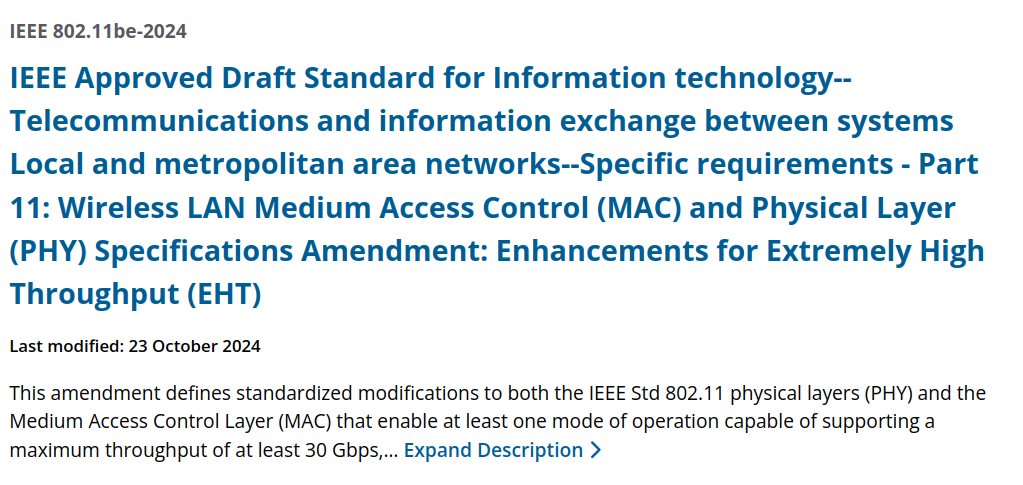
\includegraphics[width=\textwidth]{images/Ieee.png}
                \caption{Zrzut ekranu ze strony Ieee}
                \label{fig:ScIeee}
            \end{figure}
            \FloatBarrier
            \begin{figure}[ht]
                \centering
                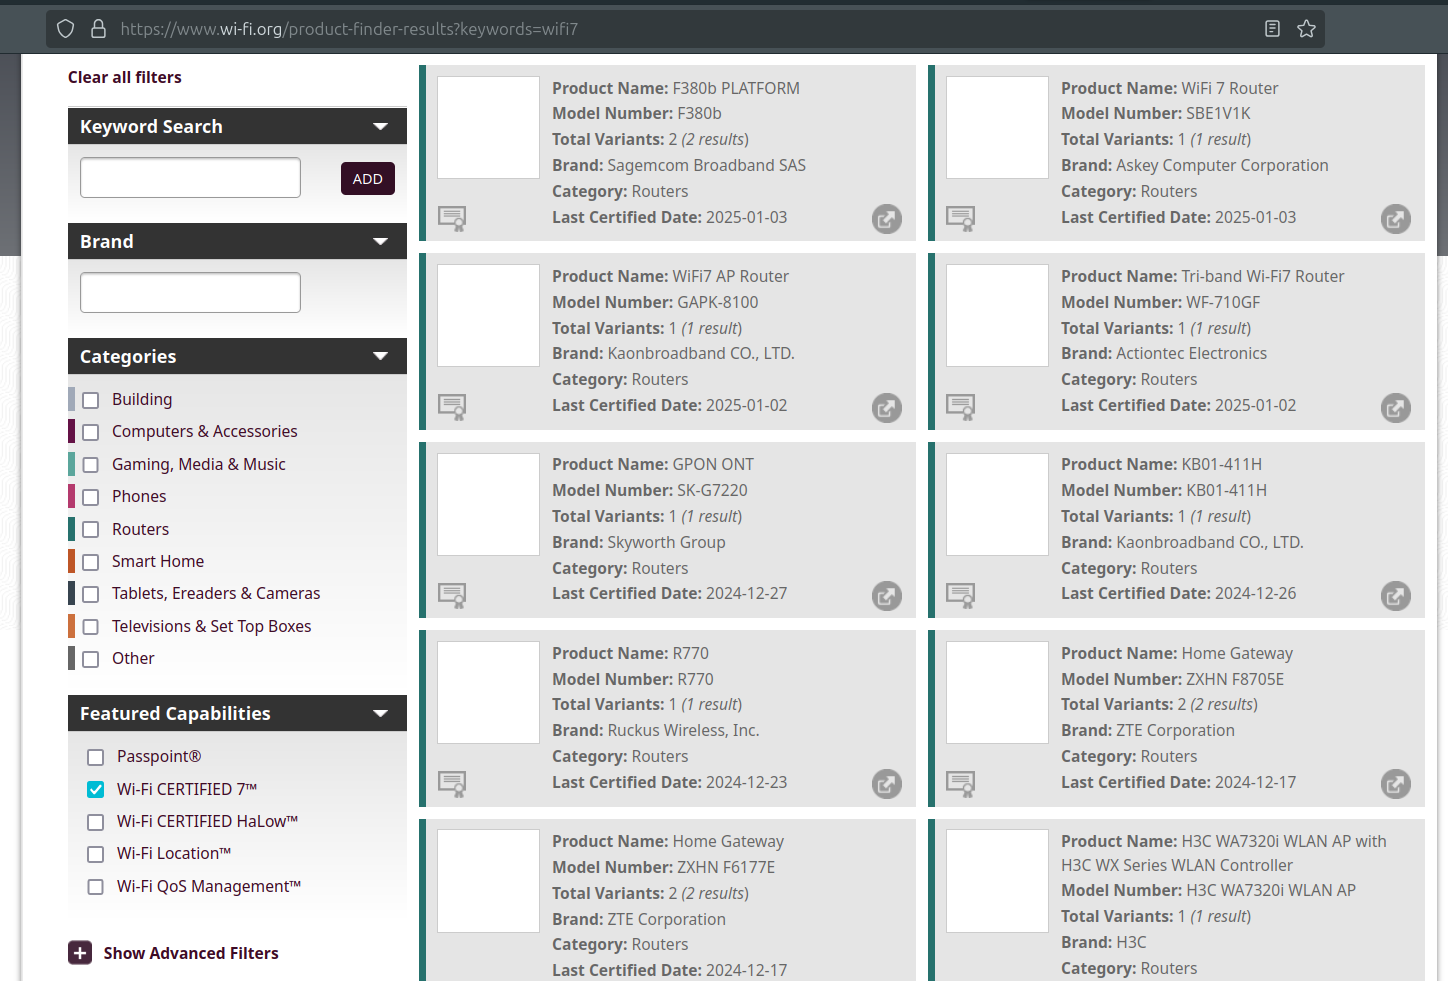
\includegraphics[width=\textwidth]{images/WiFiAcertify.png}
                \caption{Zrzut ekranu ze strony WiFi Alliance}
                \label{fig:ScWiFi}
            \end{figure}
            \FloatBarrier
        \subsection{Warstwa fizyczna}
            Standard IEEE 802.11 specyfikuje kilka protokołów warstwy fizycznej.
            \begin{enumerate}
                \item DSSS (ang. Direct Sequence Spread Spectrum) Jest techniką modulacji
                    widmem rozproszonym której szerokość pasma nadawanego jest znacznie
                    większa niż wymagana. Sygnał o małej gęstości mocy w mniejszym stopniu 
                    zakłóca działanie innych systemów na tym samym paśmie. Jako że sygnał 
                    jest wysyłany równocześnie na wielu częstotliwościach jest on 
                    redundantny i może być odtworzony mimo zakłuceń.
                \item FHSS (ang. Frequency Hopping Spread Spectrum) Jest techniką w której
                    częstotliwość nadawania zmnienia się w regularnych odstępach czasu.
                    Czas kolejnych skoków jest na tyle długi by można było przesłać kilka
                    bitów wiadomości. Widmo tego sygnału zajmuje szerokie pasmo i nie musi
                    być ciągłe co pozwala na omijanie częstotliwości. Przed transmisją 
                    nadawca i odbiorca muszą ustalić wzór skoków. 
                \item OFDM (ang. Orthogonal Frequency-Division Multiplexing) Zamiast 
                    transmitowania jednego strumienia o dużej szybkości można przesłać
                    wiele o niższej prędkości.
            \end{enumerate}
        \subsection{Kanały}
            Według standardu IEEE 802.11 zapewnione jest kilka pasm używanych w komunikacji
            WiFi. Pasma dzielą się na kanały z których kożystają poszczególne sieci. 
            Najczęściej używane pasmo to 2.4Ghz (Ma rozpiętość od 2.4Ghz do \~2.5Ghz).
            Pasmo to jest podzielone na 14 kanałów. Jednakże nie wszystkie są używane
            np w Polsce kożystamy z kanałów 1 - 13 a w USA kożysta się z kanałów 1 - 11.
            \begin{figure}[ht]
                \centering
                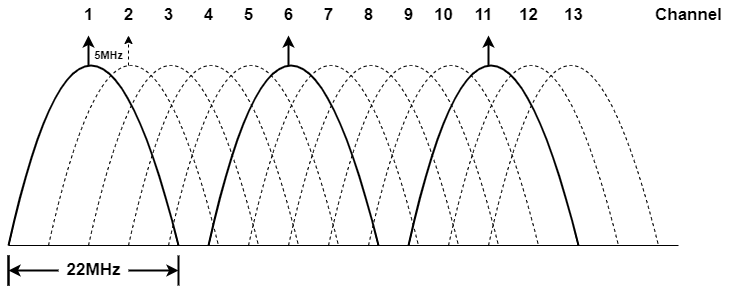
\includegraphics[width=\textwidth]{images/WiFiBands.png}
                \caption{Kanały pasma 2.4GHz}
                \label{fig:WiFiBands}
            \end{figure}
            \FloatBarrier
            Kanały są rozmieszczone co 5MHz i mają szerokość 20 MHz. Nadawanie na sąsiednich
            kanałach może powodować zakłucenia. Dlatego zaleca sięużywanie kanałów 1,6,11 
            (Ich zakres nigdy się nie pokrywa). W przypadku gdy w okolicy jest więcej niż
            trzy sieci WiFi ma kilka możliwości rozwiązania problemu.
            \begin{enumerate}
                \item Wykożystanie pasma 5GHz które ma znacznie więcej kanałów które się nie 
                    nakładają (od 19 do 23). Jednakże problemem może być krótszy zasięg.
                \item Dynamiczny wybór pasma pozwala routerowi na zmianę pasma na którym nadaje.
                \item Wykożystanie protokołu CSMA/CA (Carrier Sense Multiple Access with 
                    Collision Avoidance) router sprawdza czy pasmo z którego chce skożystać 
                    jest zajęte i w razie potrzeby czeka na "swoją kolej".
            \end{enumerate}
    \section{Zadanie laboratoryjne}
        \subsection{Treść zadania}
            W ramach zadania laboratoryjnego należało skonfigurować router WiFi, uruchomić układ SoC.
            Następnie należało napisać program dzięki któremu można będzie:
            \begin{enumerate}
                \item Włączyć i wyłączyć urządzenie
                \item Uruchomić transmisję WiFi
                \item Połączyć się z wybranym urządzeniem WiFi
                \item Przesłać dane za pomocą WiFi
            \end{enumerate}
        \subsection{Opis działania programu}
            Program wyszukuje wszystkie dostępne sieci WiFi i wypisuje ich ssid. Następnie łączy się 
            z siecią o ssid maszt\_sygnalowy. Po poprawnym połączeniu włączany jest serwer na porcie 21.
            Następnie na serwer wysyłana jest prosta strona https na której rysuje się trójkąt.
        \subsection{Schemat sieci}
            \begin{figure}[ht]
                \centering
                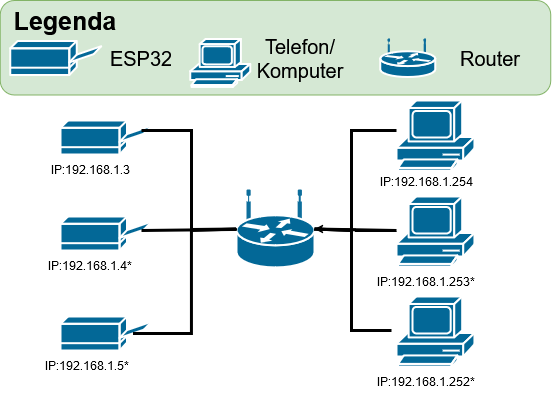
\includegraphics[width=\textwidth]{images/SiecUp.png}
                * \textit{Na zajęciach podłączony był jeden układ ESP32 i jeden telefon ale
                powinna być możliwość dodania wielu urządzeń.}
                \caption{Schemat sieci}
                \label{fig:WiFiScheme}
            \end{figure}
            \FloatBarrier
            \textbf{Dane sieci:}
            \begin{enumerate}
                \item \textbf{Nazwa:} maszt\_sygnalowy
                \item \textbf{Kanał:} 6
                \item \textbf{IP:} od 192.168.1.1 do 192.168.1.255
                \item \textbf{Adresy:} 253 (-1 adres sieci,-1 adres bramy domyślnej,-1 adres rozgłoszeniowy) 
                \item \textbf{Maska:} 255.255.255.0
                \item \textbf{Brama domyślna:} 192.168.1.2
                \item \textbf{Urządzenia ESP32:} na adresach 192.168.1.3 do 192.168.128(rosnąco)
                \item \textbf{Urządzenia klienckie:} na adresach 192.168.1.254 do 192.168.129(malejąco)
            \end{enumerate}
        \subsection{Kod programu}
            \begin{frame}
                \scriptsize
                \inputminted[
                    style={vs},
                    breaklines,
                    breakanywhere, 
                    linenos, 
                    tabsize=4 
                ]{c++}{Lab5.cpp}
                \vspace{1em}
                \captionof{listing}{Fragment kodu z programu}
                \label{lst:code}
            \end{frame}
    \section{Wnioski}
    \section{Źródła}
        \begin{enumerate}[label=\arabic*.]
            \item \url{https://www.wi-fi.org/discover-wi-fi}
            \item \url{https://standards.ieee.org/ieee/802.11be/7516/}
            \item \url{https://www.youtube.com/watch?v=QSq1TYTiESA}
            \item \url{https://www.tp-link.com/pl/support/faq/4309/}
            \item \url{https://www.audyt-wifi.pl/index.php/2024/04/05/kanaly-wifi-w-europie-sa-inne-niz-w-usa/}
            \item \url{https://www.dipol.com.pl/warstwy_fizyczne_w_standardzie_ieee_802_11_bib511.htm}
        \end{enumerate}
\end{document}